\chapter{Background}
\label{ch:Background}

In this chapter we will explore how other researchers have tackled the same problem and the valuable strategies, techniques, and knowledge discovered from their experiments.

This background research was one of the first steps in the project's life-cycle and was instrumental in better understanding this previously unknown problem which included complex chemical and medical concepts, while also introducing us to key machine learning concepts and best practices.

Due to the important nature of the problem, as discussed in Section \ref{sec:Motivation}, there have been numerous attempts to construct classification and regression machine learning models using a variety of different methods, techniques, chemical properties and other characteristics that can be extracted from the drugs themselves, such as the drug's side effects and indications, what illness they treat. \citep{Singh2020,Saber2020,Zhao2007,Gao2017,Zhang2008}. 

 Classification models, being the ones that are more widely used, try to predict whether a particular compound or drug can pass the blood-brain barrier (BBB+) or not (BBB-), and Regression models try to predict the ratio between the concentration of a compound in the brain compared to the one in the blood. This ratio is called the Brain/Plasma ratio, but studies, more often than not, use its logarithmic version called logBB.

\section{Traditional Approach Utilising Chemical Descriptors}

The classic approach to solve the problem through the creation of classification models, as showcased by \citet{Singh2020}, and regression models, as showcased by \citet{Zhang2008}, was through the usage of special software that would use the SMILES notation of a drug or compound, that essentially describes its unique chemical structure, to produce thousands, if not more, chemical descriptors. Some of these special software included \citet{Molconn-Z}, \citet{MOE}, \citet{Dragon}, used by \citet{Zhang2008} and PaDEL-Descriptors \citep{Yap2011}, used by \citet{Singh2020}. Even if the descriptors with low predictive ability were removed, just as it was done in the case of \citet{Singh2020}, hundreds of descriptors would still be left. These descriptors would then be used to train the various models.

Both \citet{Singh2020} and \citet{Zhang2008} concluded that a 
consensus model would provide superior predictive ability than a single model. This is because a consensus model combines multiple models and therefore mitigates overfitting problems associated with a single model. However, it naturally requires more computational power.

\subsection{Applicability Domain}

\citet{Zhang2008} used a very interesting concept called applicability domain (AD) which essentially calculated the "Euclidean distance between each compound and its k-nearest neighbours" and compared it with a threshold, and if it exceeded that threshold, the prediction for that specific compound would not be made.
 
 However, a case could be made that this takes away from the aim of building a predictive system used to test existing but also new drugs, drugs that could potentially be vastly different from their predecessors, leading to a large euclidean distance.

\subsection{Pitfalls}

The main pitfall to this traditional approach was the usage of special software that produced a massive number of descriptors, slowing down the models' training times while providing minimal improvements to performance as discussed by \citet{Zhao2007}. Furthermore, the usage of these special, not widely available software would also make it very difficult for someone to use the created models to make predictions without having access to the specific one used to train them.

\subsection{Improvements}

\citet{Zhao2007} aimed to reduce the high number of descriptors needed to train classification models and using Algorithm Builder, a program developed by PharmaAlgorithms Inc, 19 molecular descriptors were calculated, showcased in Table \ref{tbl:Important_Chemical_Descriptors}. Small subsets of these descriptors were then used to train different models that achieve high predictive ability, effectively making the case that small numbers of descriptors are enough to create successful models.

The findings of \citet{Zhao2007} were further confirmed by \citet{Saber2020}, making use of the same data set and choosing a subset of 8 uncorrelated chemical descriptors from the 19 previously used (Labelled as 6, 7, 8, 10, 11, 12, 13 and 19 in Table \ref{tbl:Important_Chemical_Descriptors}). It again proved that highly predictive models could be constructed using a tiny number of descriptors. These highly efficient combinations were uncovered through the use of sequential feature selection (SFS) and genetic algorithms (GA), with the study concluding that GA is a more robust approach than SFS in choosing the most relevant chemical descriptors.

Choosing a small number of highly predictive and widely available chemical descriptors leads to improved model training times and predictive performances.

\begin{table}[!ht]
  \caption{Table taken from \citet{Zhao2007} showcasing the 19 different chemical descriptors calculated.}
  \label{tbl:Important_Chemical_Descriptors}
  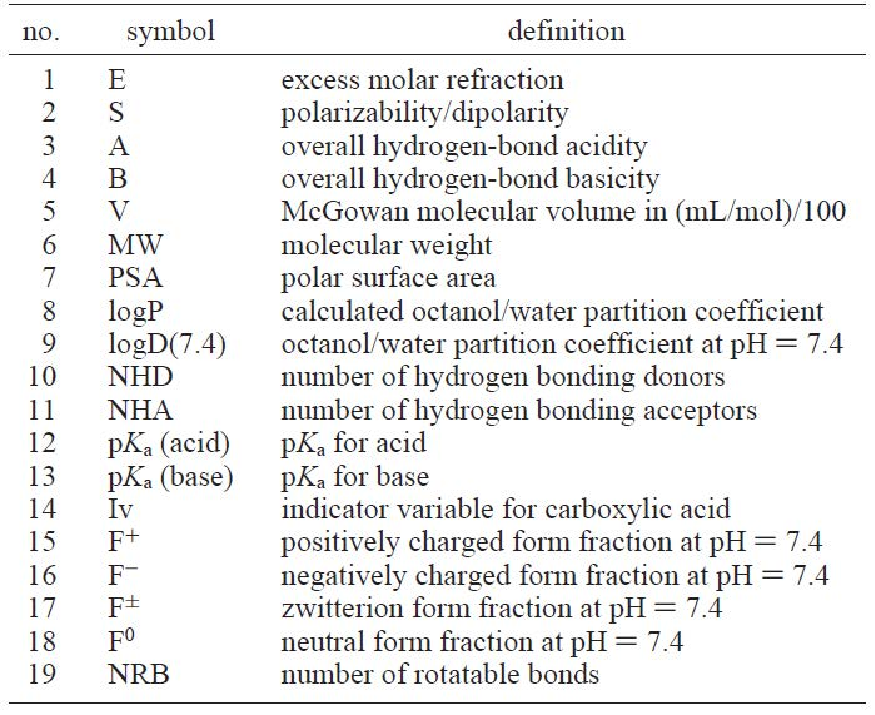
\includegraphics[width=0.55\linewidth]{images/Zhao_Table1.pdf}
\end{table}

\newpage

\section{Novel Approach Utilising Side Effects \& Indications}
\label{sec:Novel_Approach}

\citet{Gao2017} combined the usual approach of using the chemical characteristics of a drug or compound in order to predict its brain permeability with a new approach that makes use of their well-recorded side effects and indications found in the \citet{SIDER} database. 

As mentioned in Section \ref{sec:Motivation}, some larger molecules can pass into the brain using methods other than passive diffusion. These methods cannot be accurately described by the chemical characteristics of a drug or compound, but their recorded side effects and indications can capture them.

The side effects and indications were mapped to 43 subgroups, and SVM classification models were trained using multiple kernels. When both chemical descriptors and side effects and indications were available and combined, the models achieved significantly better performance than those based solely on the chemical descriptors, as showcased by Table \ref{tbl:Gao_Model_Comparison}

The study also used their created models on the \citet{SIDER} database and identified 110 drugs that can potentially penetrate the blood-brain barrier and 1018 that potentially cannot.

\begin{table}[!ht]
  \caption{Table taken from \citet{Gao2017} showcasing the different model metrics when utilising the chemical descriptors, the clinical phenotypes (meaning the side effects and indications), and a combination of the two. There seems to be a substantial increase in performance for the model utilising the combination of the two. *Prediction here means the average score achieved by cross-validation}
  \label{tbl:Gao_Model_Comparison}
  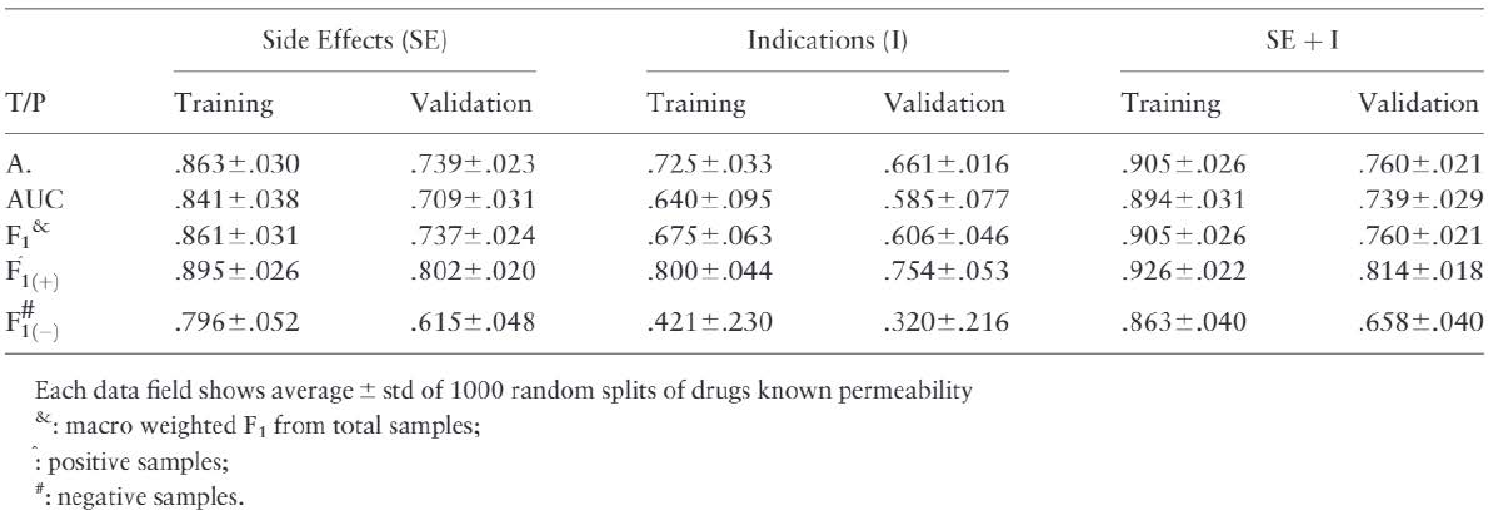
\includegraphics[width=1.0\linewidth]{images/Gao_Table_4.pdf}
\end{table}

\section{Important Chemical Descriptors}
\label{sec:Important_Chemical_Descriptors}

\citet{Zhang2008} after analysing the most frequent and vital descriptors, discovered that Polar surface area (PSA), Octanol/Water partition coefficient (logP) and the number of hydrogen bond donors and acceptor atoms were found to dominate the models. These findings were further confirmed and improved by the correlation study conducted by \citet{Zhao2007} which concluded that hydrogen-bonding properties (Labelled as 6-19 in Table \ref{tbl:Important_Chemical_Descriptors}) played a huge part in modelling brain permeability.

\citet{Singh2020} also illustrated the ranges that some of these crucial descriptors need to be within to successfully penetrate the blood-brain barrier and have an effect on the central nervous system (CNS), as showcased by Table \ref{tbl:Important_descriptors_ranges}.

However, it should be noted that even though CNS activity strongly implies BBB+, this cannot be said for the other way around, as BBB+ drugs and compounds can have no effect on the CNS.

\begin{table}[!ht]
  \caption{Table taken from \citet{Singh2020} showcasing the ranges that the most important chemical properties need to be within in order to be able to penetrate the blood-brain barrier and have an effect on the central nervous system}
  \label{tbl:Important_descriptors_ranges}
  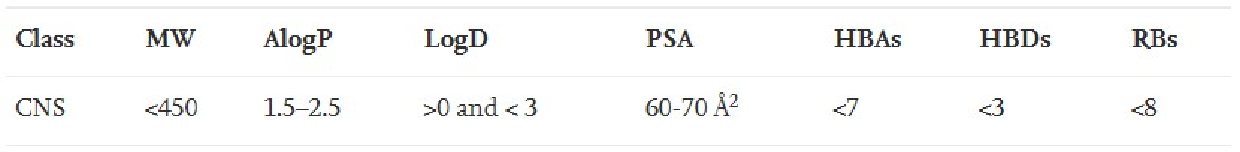
\includegraphics[width=1.0\linewidth]{images/Singh_Table1.pdf}
\end{table}

\section{Important Substructures}

\citet{Singh2020} discovered a list of corroborated substructures, as showcased in Table \ref{tbl:Substructure_Analysis}, that were more prevalent in BBB+ compounds and drugs. Even though this was something out of the scope for this project, future studies could possibly find this information helpful.

\begin{table}[!ht]
  \caption{Table taken from \citet{Singh2020} showcasing fragment occurrence in BBB+ and BBB- compounds.}
  \label{tbl:Substructure_Analysis}
  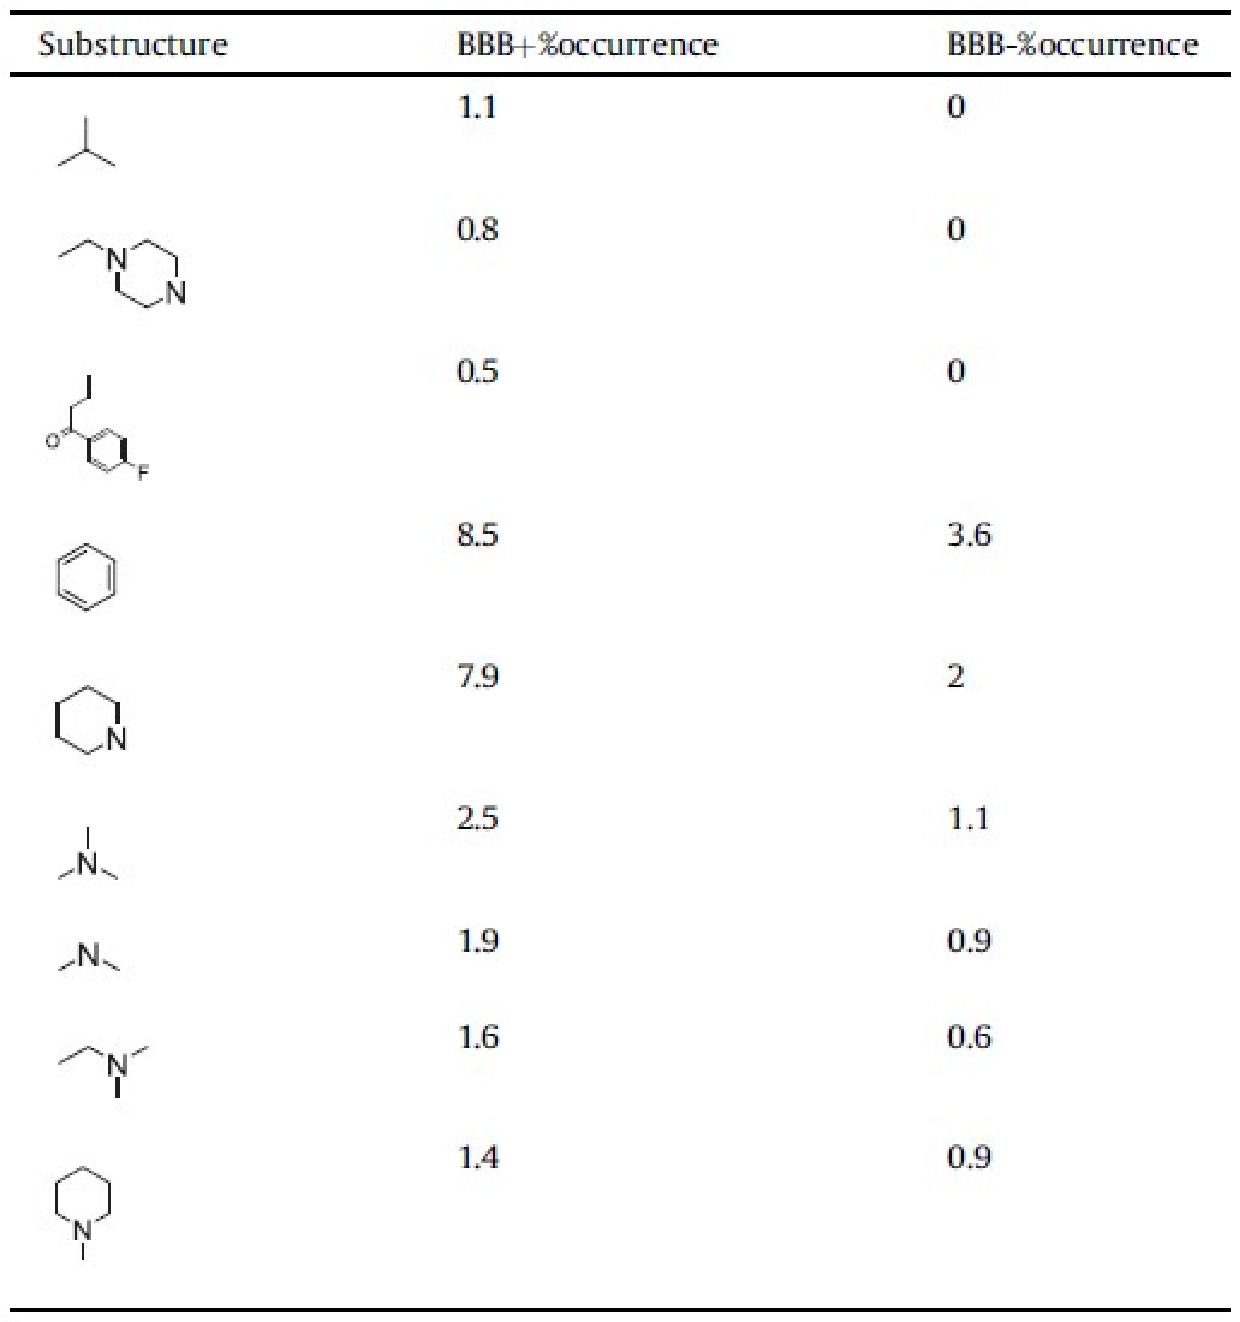
\includegraphics[width=0.45\linewidth]{images/Singh_Table13.pdf}
\end{table}

\section{Valuable Strategies \& Concepts Discovered}

All papers highlighted the importance of gathering as big a data set as possible, checking the robustness and statistical significance of models, and using holdout test sets to evaluate model predictive performance. 

The usage of small data sets leads to models not generalising effectively for unseen drugs or compounds outside their chemical space and thus making them unsuitable for high-throughput screening (HTS), which is the main objective of building such a system \citep{Singh2020}.

\citet{Zhang2008} also introduced us to the bias problem that can be caused by a class imbalance in the data set, which is often the case. This is due to the fact that most researchers are trying to discover drugs and compounds that can successfully penetrate the brain and not the other way around, naturally leading to a higher number of drugs and compounds that can enter the brain vs those that cannot, which then leads to a much higher predictive ability for the BBB+ class.


% Notes to add if needed
%\citet{Singh2020} trained Random Forest (RF), Multilayer Perceptron (MLP) and Sequential Minimal Optimisation (SMO) models.

%using two different Brain/Plasma ratio thresholds to determine whether a drug or compound can penetrate the blood-brain barrier or not.
%$$Threshold-1: Brain/Plasma \geq 0.6 \text{ as BBB+ and }Brain/Plasma < 0.6  \text{ as BBB-} $$
%$$Threshold-2: Brain/Plasma > 0.6 \text{ as BBB+ and } Brain/Plasma < 0.3 \text{ as BBB-} $$